\chapter{Results of the experiments}
\label{chap:exp}

\section{Flow eviction timeout}
\label{res:eviction-timeout}
\todo{fix plot scaling}

\begin{figure}
    \centering
    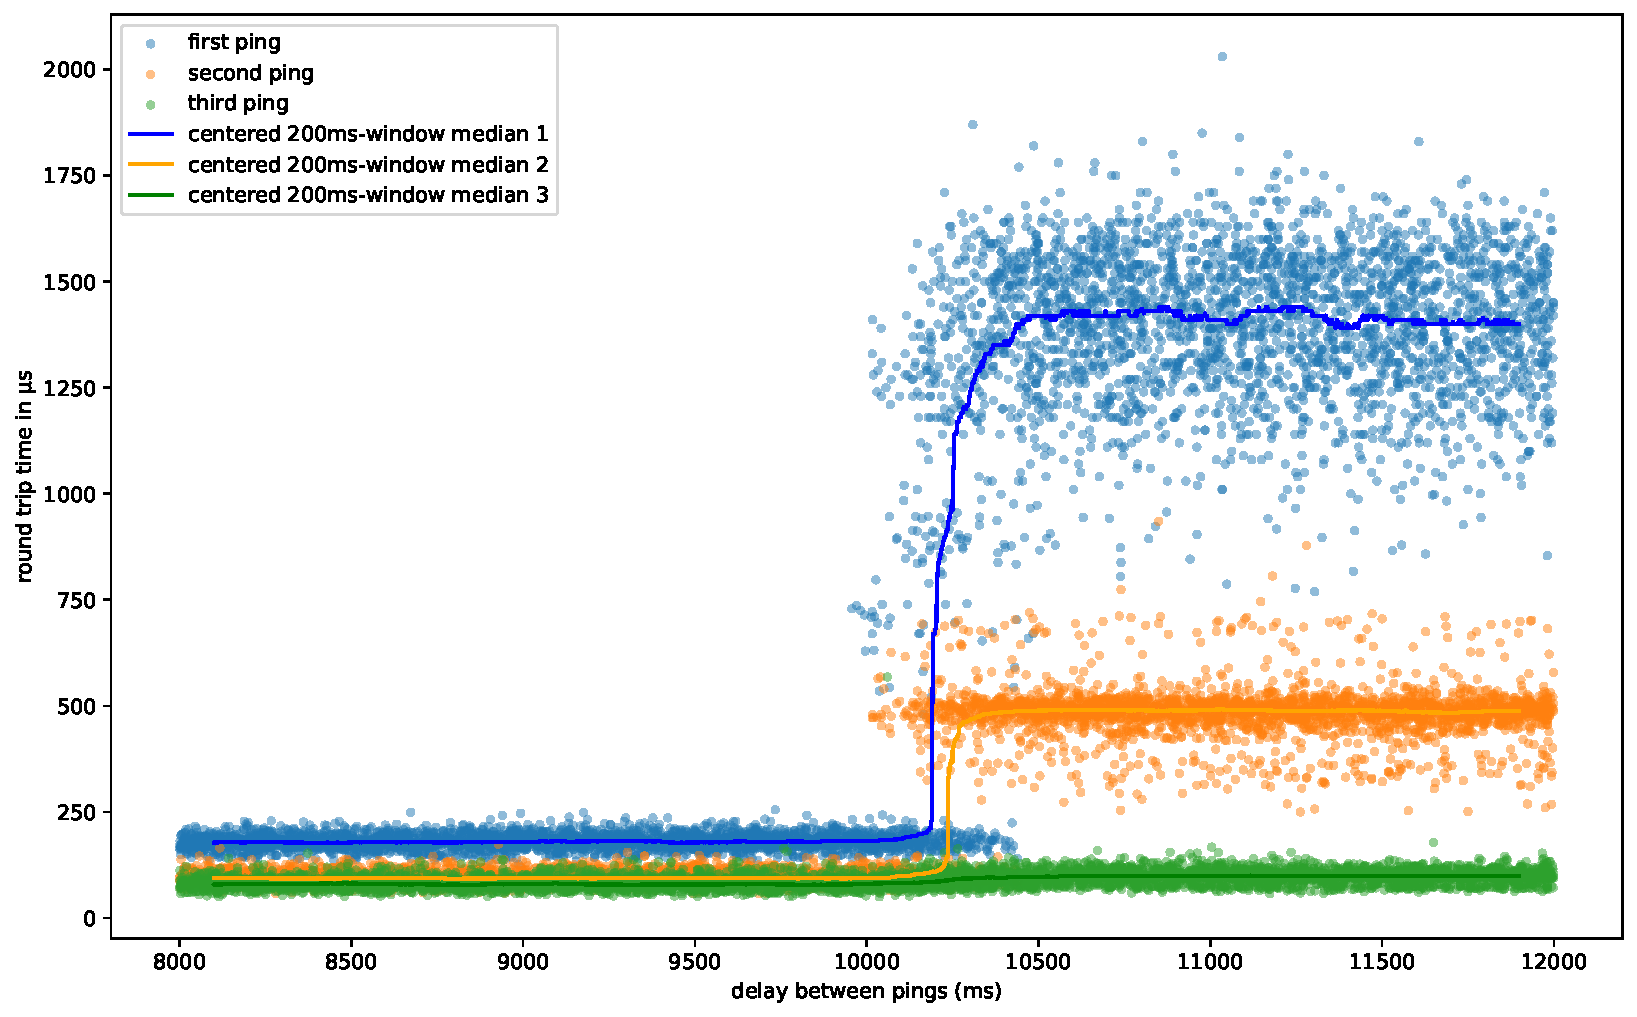
\includegraphics[width=.9\linewidth]{img/randomized_eviction_timeout.pdf}
    \caption{Results of the eviction timeout experiment with cropped outliers}
    \label{fig:plot-eviction-timeout}
\end{figure}

\paragraph{The timeout} The measured latencies of the experiment (\cref{fig:plot-eviction-timeout}) show the flow rule eviction taking effect between $10$ and $10.5$ seconds after the datapath rule installation. We assume that the timeout in software is $10$ seconds, and infrequent eviction runs cause the additional delay.

The experimental findings are consistent with the source code. In OVS's source code, the default rule timeout defined in the file \ident{ofproto/ofproto.h} as 10 seconds:
\begin{verbatim}
#define OFPROTO_MAX_IDLE_DEFAULT 10000 /* ms */
\end{verbatim}

The file \ident{ofproto/ofproto-dpif-upcall.c} contains code enforcing the timeout in the function \ident{revalidate()}:

\begin{verbatim}
if (kill_them_all || (used && used < now - max_idle)) {
    result = UKEY_DELETE;
}
\end{verbatim}

\paragraph{Difference in latency below timeout}
The results show an increased latency for the first ping compared to the second ping even when the flow rule is already installed in the datapath. We attribute this behavior to CPU caches and the internal datapath caching of rule lookups. \todo{link to explanation}


\paragraph{Increase in latency of the second ping} The measured data show another unexpected OVS behavior. The second round trip time increases when the interval is longer than the timeout by about 250 \si{\micro\second}. We do not know how to explain it.\todo{any ideas?}


\section{Cost of an upcall}
\label{res:upcall-cost}
\todo{consider joining with the previous section}

\paragraph{Cost of an upcall}
The measured data also show the cost of an upcall. The difference between round trip time without an upcall and with an upcall is around $1$ \si{\milli\second}. More precisely:

\begin{table}[h!]
    \begin{center}
        \caption{Statistics of measured round trip times when the interval }
        \label{tab:upcall-cost}
        \begin{tabular}{r|cc}
            & \textbf{First ping RTT} & \textbf{Second ping RTT} \\
            \hline
            \textbf{\#samples} & ?? & ?? \\
            \textbf{Mean} & ?? & ??\\
            \textbf{Variance} & ?? & ?? \\
            \textbf{25th percentile} & ?? & ??  \\
            \textbf{Median} & ?? & ??\\
            \textbf{75th percentile} & ?? & ?? \\
        \end{tabular}
    \end{center}
\end{table}
